\documentclass[xcolor={dvipsnames}]{beamer}
% `slidenumber' turns on slide numbering
% `hashtag=(string)` changes the hashtag, defaults to `mrg'
\usetheme[slidenumber,hashtag=ras]{iclpt}
\usepackage{roboto} % Use for fonts magic if using xelatex instead of pdflatex
\usepackage{graphicx}
\usepackage{listings}
\usepackage[{framemethod=TikZ}]{mdframed}
\usepackage{tikz}
\usepackage[dvipsnames]{xcolor}

% Colours

\colorlet{gray-bg}{Gray!5}
\colorlet{gray-title-bg}{Gray!20}
\colorlet{process-bg}{Blue!10}
\colorlet{worker-bg}{Gray!10}

\usepackage[framemethod=TikZ]{mdframed}
\usepackage{tikz}
% Named process/protocol lstlisting using mdframed+tikz package.
%

\makeatletter
\def\mdf@@codeheading{Unnamed \lstlistingname}
\define@key{mdf}{title}{\def\mdf@@codeheading{#1}}

\tikzstyle{lstnamed-label} = [
  fill=Gray,
  text=white,
  left,
  anchor=north east,
  font=\bfseries\sffamily\small,
  rounded corners=0pt,
]
\mdfdefinestyle{lstnamed}{%
    innertopmargin=3pt,
    middlelinewidth=0.5pt,
    middlelinecolor=gray-bg,
    backgroundcolor=gray-bg,
    outerlinewidth=0pt,
    outerlinecolor=white,
    innerleftmargin=0pt,
    innerrightmargin=0pt,
    innerbottommargin=0pt,
    leftmargin=0pt,
    rightmargin=0pt,
    skipabove=\topskip,
    skipbelow=\topskip,
    roundcorner=2pt,
    singleextra={\node[lstnamed-label] at (P) {\csname mdf@@codeheading\endcsname};},
    firstextra={\node[lstnamed-label]  at (P) {\csname mdf@@codeheading\endcsname};}
}

\lstnewenvironment{lstnamed}[2][]{%
  \lstset{#1}\mdframed[style=lstnamed,title={#2}]
}{\endmdframed}

%
% Default settings for tikz
%

\usetikzlibrary{arrows,calc,positioning,shapes,trees}

\newcommand{\tikzNodeText}[1]{\begin{tabular}{l}#1\end{tabular}}
\tikzstyle{process} = [
  %circle,draw,thick,fill=blue!10,
  circle,
  draw,
  fill=blue!10,
 % top color=blue!10,
 % bottom color=blue!35,
  font=\sffamily\bfseries,
  align=center,
]
\tikzstyle{process-long} = [
  %ellipse,draw,thick,fill=blue!10,
  rectangle,
  rounded corners,
  draw,
  fill=blue!10,
 % top color=blue!10,
 % bottom color=blue!35,
  font=\sffamily\bfseries\footnotesize,
  align=center,
  minimum width=4.2em,
  minimum height=2em,
]
\tikzset{
  invisible/.style={opacity=0},
  alt/.code args={<#1>#2#3}{%
    \alt<#1>{\pgfkeysalso{#2}}{\pgfkeysalso{#3}} 
  },
  visible on/.style={alt=#1{}{invisible}},
}

%
% Default settings for lstlisting
%

\newcommand{\lstCodeSize}{\footnotesize}
\newcommand{\lstPrimitiveStyle}{\color{Blue}\bfseries}
\newcommand{\lstDatatypeStyle}{\color{OliveGreen}\bfseries}
\newcommand{\lstConstStyle}{\color{RedViolet}\bfseries}
\newcommand{\lstAuxStyle}{\color{RedViolet}}
\newcommand{\lstNumberStyle}{\tiny\sffamily\color{Gray}}
\newcommand{\lstInlineStyle}{\footnotesize\ttfamily}

\lstset{
  float=hbp,
  backgroundcolor=\color{gray-bg},
  basicstyle=\lstCodeSize\ttfamily,
  identifierstyle=\color{Black},
  stringstyle=\color{Violet},
  commentstyle=\itshape\color{Gray},
  keywordstyle=\lstPrimitiveStyle,
  columns=flexible,
  tabsize=2,
  extendedchars=true,
  captionpos=b,
  numberstyle=\lstNumberStyle,
  numbers=left,
  xleftmargin=2em, % Don't go over the borders
  framexleftmargin=1.5em,
  showstringspaces=false,
  escapeinside={/*<}{>*/},
  mathescape=true,
  breaklines=true,
}
\lstdefinestyle{intable}{
  backgroundcolor=,
  numbers=none,
  breaklines=true,
  escapeinside={/*<}{>*/},
  columns=flexible
}
\lstdefinestyle{process}{
  frame=l,
  backgroundcolor=\color{gray-bg},
  numbers=none,
  breaklines=true,
  escapeinside={/*<}{>*/},
  columns=flexible,
  xleftmargin=0pt,
  framexleftmargin=0pt,
  linewidth=0.8\textwidth
}

%
% Macros for MPI listing
% Depends: lstlisting, xcolor[dvipsnames]
%

\lstdefinelanguage{MPI}{
  language=C,
  morekeywords=[2]{ % [2] Primitive keywords
    MPI_Send,
    MPI_Recv,
    MPI_Isend,
    MPI_Irecv,
    MPI_Barrier,
    MPI_Bcast,
    MPI_Reduce,
    MPI_Gather,
    MPI_Scatter,
    MPI_Allgather,
    MPI_Alltoall,
    MPI_Alltoallv,
    MPI_Allreduce,
    MPI_Probe,MPI_Iprobe,
    MPI_Comm_rank,
    MPI_Comm_size,
    MPI_Wait,
    MPI_Waitall,
    MPI_Init,
    MPI_Finalize
  },
  morekeywords=[3]{ % [3] MPI enums
    MPI_CHAR,
    MPI_UNSIGNED_CHAR,
    MPI_BYTE,
    MPI_SHORT,
    MPI_UNSIGNED_SHORT,
    MPI_INT,
    MPI_UNSIGNED,
    MPI_LONG,
    MPI_UNSIGNED_LONG,
    MPI_FLOAT,
    MPI_DOUBLE,
    MPI_LONG_DOUBLE,
    MPI_LONG_LONG_INT,
    MPI_MIN,
    MPI_PROD,
    MPI_MAX,
    MPI_MIN,
    MPI_SUM,
    MPI_PROD,
    MPI_LAND,
    MPI_BAND,
    MPI_LOR,
    MPI_BOR,
    MPI_LXOR,
    MPI_BXOR,
    MPI_MINLOC,
    MPI_MAXLOC,
  },
  morekeywords=[4]{ % [4] Types and constants with special meaning
    MPI_ANY_RANK,
    MPI_ANY_TAG,
    MPI_COMM_WORLD,
    MPI_TAG,
    MPI_Datatype,
    MPI_Op,
  },
  keywordstyle=[2]{\lstPrimitiveStyle},
  keywordstyle=[3]{\lstDatatypeStyle},
  keywordstyle=[4]{\lstConstStyle}
}

%
% Inline MPI (\lstmpi{code})
%
\newcommand\lstmpi[0]{\lstinline[language=MPI,basicstyle=\lstInlineStyle]}

%
% Macros for Pabble listing
% Depends: lstlisting, xcolor[dvipsnames], macros/lstlisting.defaults
%

\lstdefinelanguage{Scribble}{
  morekeywords={role,global,local,import,at,protocol,to,from,rec,par,choice,or,continue,package,repeat},
  morekeywords=[2]{int,float,char,string},
  keywordstyle=[2]\lstDatatypeStyle,
  morecomment=[n]{/*}{*/},
  morecomment=[l]{//},
}

%
% Macros for Pabble listing
% Depends: lstlisting, xcolor[dvipsnames], macros/lstlisting.defaults, macros/lstlisting.Scribble
%

\lstdefinelanguage{Pabble}{
  language=Scribble,
  morekeywords={if,foreach,const,range,allreduce,allgather,group,All,oneof,repeat,module},
  morekeywords=[2]{max}, % Datatype and special values
  morekeywords=[3]{inv,apply}, % Auxiliary functions
  keywordstyle=[2]\lstDatatypeStyle,
  keywordstyle=[3]\lstAuxStyle,
}

%
% Inline Pabble and Scribble (\lstscribble{code})
%
\newcommand{\lstscribble}{\lstinline[language=Pabble,basicstyle=\lstInlineStyle,mathescape]}



\title{Pabble, Session Types\\ and dataflow programming}
\author[Nicholas Ng]{Nicholas Ng\\ Mobility Reading Group}
\date{RA Symposium, 11 Jun 2015}

\newcommand{\bib}[1]{\textcolor{black!60}{\footnotesize [#1]}}

\begin{document}
\maketitle

\section{Introduction}

\frame{\frametitle{This talk}\tableofcontents[subsectionstyle=show]{}}

\begin{frame}{Problem}
  \begin{center}
  {\Large I have a tool/theory/abstraction for describing
    \textbf{communication}.\\
    Can I adapt it to describe \textbf{computation}?}
    \vfill
  \uncover<2>{\footnotesize Theoretically, $\lambda$-calculus can be encoded in
  $\pi$-calculus, but I don't program in $\pi$-calculus..}
  \end{center}
\end{frame}

\section{Session Types}

\begin{frame}{My research}
  Currently
  \begin{itemize}
    \item Practical applications of \textit{Session Types} (esp. in HPC)
    \item Tooling support for session-based programming models
    \item New ways of using the Session Types abstraction
  \end{itemize}
  Previously
  \begin{itemize}
    \item Static verification of distributed applications
    \item Code generation: Distributed parallel (MPI) applications
  \end{itemize}
\end{frame}

\subsection{Data types}

\begin{frame}[fragile]{(Data) types}
\begin{minipage}{0.50\textwidth}
\begin{lstlisting}[language=MPI]
int number = 42;        // OK
int number = add(1, 13);// OK
int number = "Nick";    // Error!
\end{lstlisting}
\end{minipage}
\begin{minipage}{0.46\textwidth}
  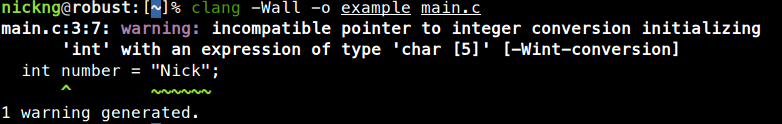
\includegraphics[width=\linewidth]{type-error}

  {\footnotesize Type error reported by compiler}
\end{minipage}
%
\begin{block}<1>{Types}
  \begin{tabular}{lll}
                                         & \textbf{Expression/statement} & \textbf{Type} \\
    variable                             & \lstmpi{number}               & \lstmpi{int} (integer)\\
    value                                & \lstmpi{52}                   & \lstmpi{int}\\
    function call (returns \lstmpi{int}) & \lstmpi{add(1, 13)}           & \lstmpi{int}\\
    value                                & \lstmpi{"Nick"}               & \lstmpi{char}s\\
  \end{tabular}
\end{block}
%\begin{center}
% $\Gamma \vdash P \vartriangleright \Delta$\\
% \textit{Under the environment $\Gamma$, Process $P$ has typing $\Delta$}.
%\end{center}
\end{frame}

\subsection{Session types}
\begin{frame}{Session Types: Intuition} % -----------------------------------------------
  \begin{itemize}
    \item Traditional (data) types
      \begin{itemize}
        \item Data types: \textcolor{red}{int} $\longleftrightarrow$ \textcolor{blue}{int}
        \item Makes sure the variable and the value are \textbf{compatible}
        \item Useful to abstract and proof properties of a \textbf{program}
      \end{itemize}
    \item<2> Session Types
      \begin{itemize}
        \item \textit{Types for communication} (e.g.~message-passing send/recv)
        \item Communication always involves two sides
        \item Session types: \textcolor{red}{send} $\longleftrightarrow$ \textcolor{blue}{receive}
        \item Types across two processes, i.e.~types for communication
        \item Makes sure the communication is \textbf{compatible}
        \item Useful to abstract and proof properties of a \textbf{communication}
      \end{itemize}
  \end{itemize}
\end{frame}

\begin{frame}{Session Types}
  \begin{flushright}
    \textcolor{gray}{\textit{\scriptsize It's an abstraction.. it's a verification method.. It's Session Types!}}\\
  \end{flushright}
  Sessions
  \begin{itemize}
    \item Session Type refers to the type of the whole program
    \item A series of send/receive with control-flow structure
    \item Abstraction for structured communication: a.k.a. \textit{communication protocol}
  \end{itemize}
  But how do we use it?
\end{frame}

\begin{frame}{Session Types in practice}
  \begin{block}{Theory}
  \begin{center}
    Binary Session Types \bib{PARL'94,ESOP'98}\\
    $\downarrow$\\
    Multiparty Session Types (MPST) \bib{POPL'08}\\
    $\downarrow$\\
    Parameterised Multiparty Session Types \bib{FoSSaCS'10,LMCS 2012}
  \end{center}
\end{block}
Scribble project
  \begin{itemize}
    \item Protocol description language
    \item Practical realisation of Multiparty Session Types
    \item Developed with industry
  \end{itemize}

  
\includegraphics[height=2em]{ooi-logo}
  \hfill
  
\includegraphics[height=2em]{redhat-logo}
  \hfill
  
\includegraphics[height=2em]{savara-logo}
  \hfill
  
\includegraphics[height=2em]{cognizant-logo}
\end{frame}

\section{Pabble protocol language}

\begin{frame}{Pabble protocol language}
  \textbf{Pabble}: Parameterised Scribble \bib{PDP'14,SoCA 2015}
  \begin{itemize}
    \item Scribble + parameters: scalable protocols
    \item Realisation of Parameterised MPST
    \item Generate MPI code from communication patterns \bib{CC'15}
      \begin{itemize}
        \item Common, reusable \textit{patterns} (e.g. Map-Reduce)
        \item Topologies to connect parallel processes
      \end{itemize}
  \end{itemize}
  Other Scribble protocol uses
  \begin{itemize}
    \item Conformance verification \bib{TOOLS'12,EuroMPI'12}
    \item Runtime monitoring \bib{COORDINATION'14,FMSD 2015}
    \item and more \dots
  \end{itemize}
\end{frame}

\subsection{Example}

\tikzstyle{every picture}+=[remember picture]{
\begin{frame}[fragile]{Pabble protocol: Example}
  \begin{center}
  \begin{lstnamed}[language=Pabble]{Pabble protocol}
global protocol Ring(role P[/*<\tikz[baseline]{\node[anchor=base,inner sep=2pt,fill=teal!20](range-parameters){1..4};}>*/]) {
  rec LOOP {
    /*<\tikz[baseline]{\node[fill=violet!20,anchor=base,inner sep=2pt](foreach-loop){\textcolor{Blue}{foreach} (i:1..3)};}>*/ {
      Data(int) from /*<\tikz[baseline]{\node[fill=blue!20,anchor=base,inner sep=2pt](wi){P[i]};}>*/ to /*<\tikz[baseline]{\node[fill=red!20,anchor=base,inner sep=2pt](wi1){P[\tikz[baseline]{\node[anchor=base,inner sep=0pt](relative-index){\underline{i+1}};}]};}>*/;
    }
    Data(int) from /*<\tikz[baseline]{\node[anchor=base,inner sep=2pt,fill=orange!20](direct-participant){P[4]};}>*/ to /*<\tikz[baseline]{\node[anchor=base,inner sep=2pt](w1){P[1]};}>*/;
    continue LOOP; } }
  \end{lstnamed}
  \only<1>{
  \begin{itemize}
    \item Foreach loop over indices \tikz\node(foreach-loop-desc){};
    \item Direct participant reference \tikz\node(direct-participant-desc){};
    \item Declare roles with index range \tikz\node(range-parameters-desc){};
    \item Relative index calculation (integer arithmetic) \tikz\node(relative-index-desc){};
  \end{itemize}
  \begin{tikzpicture}[overlay]
    \path<1>[->,violet,thick] (foreach-loop-desc) edge (foreach-loop);
    \path<1>[->,orange,thick] (direct-participant-desc) edge [bend right] (direct-participant);
    \path<1>[->,teal,thick] (range-parameters-desc) edge [bend right] (range-parameters);
    \path<1>[->,red,thick] (relative-index-desc) edge [bend right] (relative-index);
  \end{tikzpicture}
  }
  \only<2>{
  \resizebox{0.8\textwidth}{!}{
  \begin{tikzpicture}
    \node[rectangle,draw,process-long] (P1) {\tt P[0]};
    \node[rectangle,draw,right=2 of P1,process-long] (P2) {\tt P[2]};
    \node[rectangle,draw,right=2 of P2,process-long] (P3) {\tt P[3]};
    \node[rectangle,draw,right=2 of P3,process-long] (P4) {\tt P[4]};
    \node[below=0.5 of P1] (P11) {};
    \node[below=0.5 of P2] (P21) {};
    \node[below=0.5 of P3] (P31) {};
    \node[below=0.5 of P4] (P41) {};
    \node[below=0.5 of P11] (P12) {};
    \node[below=0.5 of P21] (P22) {};
    \node[below=0.5 of P31] (P32) {};
    \node[below=0.5 of P41] (P42) {};
    \node[below=0.5 of P12] (P13) {};
    \node[below=0.5 of P22] (P23) {};
    \node[below=0.5 of P32] (P33) {};
    \node[below=0.5 of P42] (P43) {};
    \node[below=0.5 of P13] (P14) {};
    \node[below=0.5 of P23] (P24) {};
    \node[below=0.5 of P33] (P34) {};
    \node[below=0.5 of P43] (P44) {};
    \node[below=0.5 of P14] (P15) {};
    \node[below=0.5 of P24] (P25) {};
    \node[below=0.5 of P34] (P35) {};
    \node[below=0.5 of P44] (P45) {};
    \node[below=0.1 of P15] (P16) {};
    \node[below=0.1 of P25] (P26) {};
    \node[below=0.1 of P35] (P36) {};
    \node[below=0.1 of P45] (P46) {};
    \draw (P1.south) -- (P16);
    \draw (P2.south) -- (P26);
    \draw (P3.south) -- (P36);
    \draw (P4.south) -- (P46);
    \draw[->] (P11) edge node[midway,yshift=2mm]{\small \lstscribble{Message(int)}} (P21);
    \draw[->] (P22) edge node[midway,yshift=2mm]{\small \lstscribble{Message(int)}} (P32);
    \draw[->] (P33) edge node[midway,yshift=2mm]{\small \lstscribble{Message(int)}} (P43);
    \draw[->] (P44) edge node[midway,yshift=2mm]{\small \lstscribble{Message(int)}} (P14);
  \end{tikzpicture}
  }
  }
  \end{center}
\end{frame}
}

\subsection{Summary}

\begin{frame}{Summary: Pabble protocol language}
  Scribble/Pabble: Practical session types
  \begin{itemize}
    \item Protocols: sequences of message-passing actions
    \item Concurrency: Participants follow protocol $\rightarrow$ compatible
    \item Abstraction: Express communication patterns
      \begin{itemize}
        \item Data abstracted away
        \item Both good and bad: What about computation?
      \end{itemize}
  \end{itemize}
\end{frame}

\section{The dataflow model and dataflow programming with Pabble}

\begin{frame}{The dataflow model}
  \begin{minipage}{0.69\textwidth}
    \only<1>{
    \textit{``\footnotesize If a reaction of actor A requires data produced by a reaction of
    actor B, then the reaction of A must occur after the reaction of B. A MoC
  where such data dependencies are the key constraints on reactions is called a
dataflow model of computation."\\-- Lee and Seshia, Introduction to Embedded
Systems}
    }
    \only<2>{
      \begin{center}
        {\Huge Computation}
        model defined by the \textbf{flow structure/dependency graph of data} not control flow depending on the data.
      \end{center}
    }
  \end{minipage}
  \begin{minipage}{0.29\textwidth}
    
\includegraphics[width=\linewidth]{intro-to-embedded-systems-book-cover}
  \end{minipage}
\end{frame}

\begin{frame}{Some properties of the dataflow model}
  \begin{minipage}{0.59\textwidth}
  \begin{itemize}
    \item Data flow: data goes to all nodes
    \item Structure of the flow unchanged
    \item Data flow graph $\longrightarrow$
  \end{itemize}
  \end{minipage}
  \begin{minipage}{0.39\textwidth}
    \tikzstyle{offset} = [diamond,fill=blue!20]
    \tikzstyle{op} = [circle,fill=red!20]
    \tikzstyle{const} = [rectangle,fill=green!20]
    \begin{tikzpicture}[node distance = 2cm, auto]
      \node [const] (x) {x};
      \coordinate [left=0.5 of x] (lx);
      \coordinate [right=0.5 of x] (rx);
      \node [below=0.5 of x] (splx) {};
      \node [below=0.05 of splx] {};
      \node [offset,left=0.5 of splx] (min1) {-1};
      \node [offset,right=0.5 of splx] (plu1) {+1};
      \node [op,below=0.5 of splx] (add1) {+};
      \node [op,below=0.5 of add1] (add2) {+};
      \node [op,below=0.5 of add2] (div1) {/};
      \coordinate [left=0.5 of add1] (ladd1);
      \coordinate [right=0.5 of add2] (radd2);
      \node [const,right=0.5 of div1] (three) {3};
      \node [const,below=0.5 of div1] (y) {y};
      \path [draw=black,->] (x) -- (lx) -- (min1.north);
      \path [draw=black,->] (x) -- (rx) -- (plu1.north);
      \path [draw=black,->] (min1.south) -- (ladd1) -- (add1.west);
      \path [draw=black,->] (plu1.south) -- (radd2) -- (add2.east);
      \path [draw=black,->] (three) -- (div1.east);
      \path [draw=black,->] (add1) -- (add2.north);
      \path [draw=black,->] (add2.south) -- (div1.north);
      \path [draw=black,->] (div1.south) -- (y.north);
    \end{tikzpicture}

    {\footnotesize Example: moving average data flow kernel graph from Maxeler tutorial}
\end{minipage}
\end{frame}

\begin{frame}{Dataflow model for programming}
  Apache Storm
  \begin{itemize}
    \item ``Storm, distributed and fault-tolerant realtime computation"
    \item ASF since 2014
    \item Like \textbf{Hadoop} but for realtime processing
      \begin{enumerate}
        \item Construct \alert<2>{\textit{topology}} (connected graph of nodes)
        \item Implement \textit{Bolts} (nodes)
        \item Execute stream
      \end{enumerate}
  \end{itemize}
  Google Cloud Dataflow
  \begin{itemize}
    \item FlumeJava: Easy, Efficient Data-Parallel Pipelines \bib{PLDI'10}
    \item Java SDK out of beta last month
    \item Like \textbf{MapReduce} but better (more flexible)
      \begin{enumerate}
        \item Chain data-parallel primitives to get \alert<2>{\textit{execution plan}}
        \item Optimise execution plan (group and rearrange nodes)
        \item Execute plan
        \item Profit!
      \end{enumerate}
  \end{itemize}
\end{frame}

\begin{frame}{It's the pattern!}
  \begin{center}
    \textit{data flow graph}\qquad
    \textit{topology}\qquad
    \textit{execution plan}
  \end{center}
  \begin{itemize}
    \item Data flow graph $\longleftrightarrow$ computation
    \item Apply Session Types, protocols to data flow graph
    \item $\Rightarrow$ Session Types to describe computation
    \item $\Rightarrow$ Hierarchy of session types for
      \begin{itemize}
        \item Distributed communication
        \item Local computation
      \end{itemize}
  \end{itemize}
\end{frame}

\subsection{Example}

\begin{frame}[fragile]{Data flow programming with Pabble}
  \begin{minipage}{0.69\textwidth}
    \begin{lstnamed}[language=Pabble]{MSCR}
global protocol MSCR_Figure3(
    role Map[1..3], role GBK[1..2],
    role CV[1..2], role R[1..2]) {
  input1() from __IN to Map[1];
  input2() from __IN to Map[2];
  input3() from __IN to Map[3];
  T() from Map[1] to GBK[1], GBK[2];
  T() from Map[2] to GBK[1], GBK[2];
  output3() from Map[3] to GBK[2], __OUT;
  T() from GBK[1] to CV[1];
  T() from GBK[2] to CV[2];
  T() from CV[1] to R[1];
  T() from CV[2] to R[2];
  output1() from R[1] to __OUT;
  output2() from R[2] to __OUT;
}
    \end{lstnamed}
  \end{minipage}
  \begin{minipage}{0.29\textwidth}
    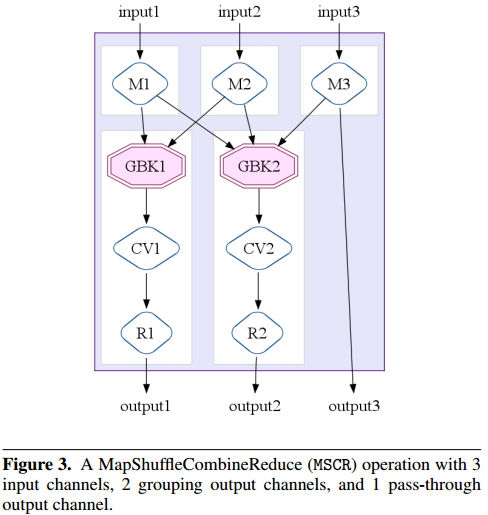
\includegraphics[width=1.2\textwidth]{mscr-3i3o}

    {\footnotesize MSCR operation with 3 input, 3 output from \bib{PLDI'10}}
  \end{minipage}
\end{frame}

\subsection{Challenges}

\begin{frame}{Challenges}
  Abstraction
  \begin{itemize}
    \item \texttt{MSCR} example is still too high level
      \begin{itemize}
        \item How do you define \texttt{Map}, \texttt{CV}, etc.
        \item Predefine common nodes?
      \end{itemize}
    \item Dataflow API for stream processors
    \item CPU hardware/embedded systems = dataflow pipelines
  \end{itemize}
  Graphical
  \begin{itemize}
    \item Easy to use (and understand)
    \item Use text to describe graphs? Not so easy
    \item Session Types and WS-CDL/BPMN
  \end{itemize}

\end{frame}

\section{Wrapping up}

\begin{frame}{Concluding remarks}
  \begin{center}
  {\Large I have a abstraction/tool/theory for describing
    \textbf{communication}.\\
    Can I adapt it to describe \textbf{computation}?}
    \vfill
    \textbf{Probably}, if we investigate using data flow programming for session
    types, and see what kinds of problems this approach can tackle.
    \vfill
    \uncover<2>{ Thank you! Feedback: \texttt{nickng@imperial.ac.uk} }
  \end{center}
\end{frame}

\begin{frame}{}
\end{frame}

\begin{frame}{Distributed Systems vs. Parallel Programming}{Also Scribble vs. Pabble}

  \begin{minipage}{0.23\textwidth}
    \centering
    \tikzset{proc/.style={draw,rectangle,inner sep=2pt,fill=white}}
    \begin{tikzpicture}
      \node [proc] (a) {\tiny Alice};
      \node [proc,right=6pt of a,xshift=10pt] (b) {\tiny Bob};
      \node [proc,below=10pt of a] (c) {\tiny Buyer};
      \node [proc,right=14pt of c,yshift=-6pt] (d) {\tiny Seller};
      \draw [->,thick] (a) -- (b);
      \draw [->,thick] (c) -- (b);
      \draw [->,thick] (a) -- (d);
      \draw [->,thick] (d) -- (a);
      \draw [->,thick] (d) -- (b);
      \draw [->,thick] (d) -- (c);
    \end{tikzpicture}
    \vskip 2em
    \begin{tikzpicture}
      \node [proc] (p0) {\tiny P[0]};
      \node [proc,right=5pt of p0] (p1) {\tiny P[1]};
      \node [right=5pt of p1] (px) {\tiny \dots};
      \node [proc,right=5pt of px] (pn) {\tiny P[1000]};
      \path [->,thick] (p0) edge [out=45,in=135] (p1);
      \path [->,thick] (p1) edge [out=45,in=135] (px);
      \path [->,thick] (px) edge [out=45,in=135] (pn);
      \path [->,thick] (pn) edge [in=315,out=225] (px);
      \path [->,thick] (px) edge [in=315,out=225] (p1);
      \path [->,thick] (p1) edge [in=315,out=225] (p0);
    \end{tikzpicture}
  \end{minipage}
  \begin{minipage}{0.755\textwidth}
    \begin{itemize}
      \item Participants identified by \textbf{names}
        \begin{itemize}
          \item e.g.~{\tt Alice}, {\tt Bob}, {\tt Buyer}, {\tt Seller}
          \item Complex interactions
          \item Between a few participants
        \end{itemize}
      \item Participants identified by \textbf{indices}
        \begin{itemize}
          \item e.g.~{\tt P[0]}, {\tt P[1]}, {\tt P[100]} {\tt P[i+1]}
          \item Structured interactions
          \item Between many participants
          \item Scalable: arithmetic operations on indices
        \end{itemize}
    \end{itemize}
  \end{minipage}
\end{frame}

\end{document}
